\documentclass[
11pt,
english,
singlespacing,
headsepline,
]{MastersDoctoralThesis}

\usepackage[utf8]{inputenc}
\usepackage[T1]{fontenc}
\usepackage{mathpazo}
\usepackage[backend=bibtex,style=authoryear,natbib=true]{biblatex}
\addbibresource{example.bib}
\usepackage[autostyle=true]{csquotes}
\usepackage{float}

%----------------------------------------------------------------------------------------
%	MARGIN SETTINGS
%----------------------------------------------------------------------------------------

\geometry{
	paper=a4paper, % Change to letterpaper for US letter
	inner=2.5cm, % Inner margin
	outer=3.8cm, % Outer margin
	bindingoffset=.5cm, % Binding offset
	top=1.5cm, % Top margin
	bottom=1.5cm, % Bottom margin
	%showframe, % Uncomment to show how the type block is set on the page
}

%----------------------------------------------------------------------------------------
%	THESIS INFORMATION
%----------------------------------------------------------------------------------------

\thesistitle{Non-Technical Generation of Object-Oriented Code}
\supervisor{Sara \textsc{Kalvala}}
\degree{Computer Science}
\author{Thomas \textsc{Allton}}
\subject{Computer Science}
\keywords{Reflection, Java, Compiler, Parser, Representation, JSON, Object-Oriented} % \keywordnames
\university{\href{https://warwick.ac.uk/}{University of Warwick}}
\department{\href{https://warwick.ac.uk/fac/sci/dcs/}{Department of Computer Science}}

\AtBeginDocument{
\hypersetup{pdftitle=\ttitle}
\hypersetup{pdfauthor=\authorname}
\hypersetup{pdfkeywords=\keywordnames}
}

\begin{document}

\frontmatter % Use roman page numbering style (i, ii, iii, iv...) for the pre-content pages

\pagestyle{plain} % Default to the plain heading style until the thesis style is called for the body content

%----------------------------------------------------------------------------------------
%	TITLE PAGE
%----------------------------------------------------------------------------------------

\begin{titlepage}
\begin{center}

\vspace*{.06\textheight}
{\scshape\LARGE \univname\par}\vspace{1.5cm} % University name
\textsc{\Large Department of Computer Science}\\[0.5cm] % Thesis type
\textsc{\large CS310: Third Year Project}\\[0.5cm] % Thesis type

\HRule \\[0.4cm] % Horizontal line
{\huge \bfseries \ttitle\par}\vspace{0.4cm} % Thesis title
\HRule \\[1.5cm] % Horizontal line
 
\begin{minipage}[t]{0.4\textwidth}
\begin{flushleft} \large
\emph{Author:}\\
\href{https://www.tomallton.com}{\authorname} % Author name - remove the \href bracket to remove the link
\end{flushleft}
\end{minipage}
\begin{minipage}[t]{0.4\textwidth}
\begin{flushright} \large
\emph{Supervisor:} \\
\href{https://warwick.ac.uk/fac/sci/dcs/people/sara_kalvala/}{\supname} % Supervisor name - remove the \href bracket to remove the link  
\end{flushright}
\end{minipage}\\[2cm]
{\large \today}\\[2cm] % Date

\includegraphics{Logo} % University/department logo
\end{center}
\end{titlepage}

%----------------------------------------------------------------------------------------
%	DECLARATION PAGE
%----------------------------------------------------------------------------------------

\begin{declaration}
\addchaptertocentry{\authorshipname} % Add the declaration to the table of contents
\noindent I, \authorname, declare that this thesis titled, \enquote{\ttitle} and the work presented in it are my own. I confirm that:

\begin{itemize} 
\item This work was done wholly or mainly while in candidature for a research degree at this University.
\item Where any part of this thesis has previously been submitted for a degree or any other qualification at this University or any other institution, this has been clearly stated.
\item Where I have consulted the published work of others, this is always clearly attributed.
\item Where I have quoted from the work of others, the source is always given. With the exception of such quotations, this thesis is entirely my own work.
\item I have acknowledged all main sources of help.
\item Where the thesis is based on work done by myself jointly with others, I have made clear exactly what was done by others and what I have contributed myself.\\
\end{itemize}
 
\noindent Signed:\\
\rule[0.5em]{25em}{0.5pt} % This prints a line for the signature
 
\noindent Date:\\
\rule[0.5em]{25em}{0.5pt} % This prints a line to write the date
\end{declaration}

\cleardoublepage

%----------------------------------------------------------------------------------------
%	QUOTATION PAGE
%----------------------------------------------------------------------------------------

\vspace*{0.2\textheight}

\noindent\enquote{\itshape Thanks to my solid academic training, today I can write hundreds of words on virtually any topic without possessing a shred of information, which is how I got a good job in journalism.}\bigbreak

\hfill Dave Barry

%----------------------------------------------------------------------------------------
%	ABSTRACT PAGE
%----------------------------------------------------------------------------------------

\begin{abstract}
\addchaptertocentry{\abstractname} % Add the abstract to the table of contents
The Thesis Abstract is written here (and usually kept to just this page). The page is kept centered vertically so can expand into the blank space above the title too\ldots
\end{abstract}

%----------------------------------------------------------------------------------------
%	ACKNOWLEDGEMENTS
%----------------------------------------------------------------------------------------

\begin{acknowledgements}
\addchaptertocentry{\acknowledgementname} % Add the acknowledgements to the table of contents
The acknowledgments and the people to thank go here, don't forget to include your project advisor\ldots
\end{acknowledgements}

%----------------------------------------------------------------------------------------
%	LIST OF CONTENTS/FIGURES/TABLES PAGES
%----------------------------------------------------------------------------------------

\tableofcontents % Prints the main table of contents

\listoffigures % Prints the list of figures

\listoftables % Prints the list of tables

%----------------------------------------------------------------------------------------
%	ABBREVIATIONS
%----------------------------------------------------------------------------------------

\begin{abbreviations}{ll} % Include a list of abbreviations (a table of two columns)

\textbf{LAH} & \textbf{L}ist \textbf{A}bbreviations \textbf{H}ere\\
\textbf{WSF} & \textbf{W}hat (it) \textbf{S}tands \textbf{F}or\\

\end{abbreviations}

%----------------------------------------------------------------------------------------
%	PHYSICAL CONSTANTS/OTHER DEFINITIONS
%----------------------------------------------------------------------------------------

\begin{constants}{lr@{${}={}$}l} % The list of physical constants is a three column table

% The \SI{}{} command is provided by the siunitx package, see its documentation for instructions on how to use it

Speed of Light & $c_{0}$ & \SI{2.99792458e8}{\meter\per\second} (exact)\\
%Constant Name & $Symbol$ & $Constant Value$ with units\\

\end{constants}

%----------------------------------------------------------------------------------------
%	SYMBOLS
%----------------------------------------------------------------------------------------

\begin{symbols}{lll} % Include a list of Symbols (a three column table)

$a$ & distance & \si{\meter} \\
$P$ & power & \si{\watt} (\si{\joule\per\second}) \\
%Symbol & Name & Unit \\

\addlinespace % Gap to separate the Roman symbols from the Greek

$\omega$ & angular frequency & \si{\radian} \\

\end{symbols}

%----------------------------------------------------------------------------------------
%	DEDICATION
%----------------------------------------------------------------------------------------

\dedicatory{For/Dedicated to/To my\ldots} 

%----------------------------------------------------------------------------------------
%	THESIS CONTENT - CHAPTERS
%----------------------------------------------------------------------------------------

\mainmatter % Begin numeric (1,2,3...) page numbering

\pagestyle{thesis} % Return the page headers back to the "thesis" style

% Include the chapters of the thesis as separate files from the Chapters folder
% Uncomment the lines as you write the chapters

% Chapter 1

\chapter{Chapter Title Here} % Main chapter title

\label{Chapter1} % For referencing the chapter elsewhere, use \ref{Chapter1} 

%----------------------------------------------------------------------------------------

% Define some commands to keep the formatting separated from the content 
\newcommand{\keyword}[1]{\textbf{#1}}
\newcommand{\tabhead}[1]{\textbf{#1}}
\newcommand{\code}[1]{\texttt{#1}}
\newcommand{\file}[1]{\texttt{\bfseries#1}}
\newcommand{\option}[1]{\texttt{\itshape#1}}

%----------------------------------------------------------------------------------------

\section{Welcome and Thank You}
Welcome to this \LaTeX{} Thesis Template, a beautiful and easy to use template for writing a thesis using the \LaTeX{} typesetting system.

If you are writing a thesis (or will be in the future) and its subject is technical or mathematical (though it doesn't have to be), then creating it in \LaTeX{} is highly recommended as a way to make sure you can just get down to the essential writing without having to worry over formatting or wasting time arguing with your word processor.

\LaTeX{} is easily able to professionally typeset documents that run to hundreds or thousands of pages long. With simple mark-up commands, it automatically sets out the table of contents, margins, page headers and footers and keeps the formatting consistent and beautiful. One of its main strengths is the way it can easily typeset mathematics, even \emph{heavy} mathematics. Even if those equations are the most horribly twisted and most difficult mathematical problems that can only be solved on a super-computer, you can at least count on \LaTeX{} to make them look stunning.

%----------------------------------------------------------------------------------------

\section{Learning \LaTeX{}}

\LaTeX{} is not a \textsc{wysiwyg} (What You See is What You Get) program, unlike word processors such as Microsoft Word or Apple's Pages. Instead, a document written for \LaTeX{} is actually a simple, plain text file that contains \emph{no formatting}. You tell \LaTeX{} how you want the formatting in the finished document by writing in simple commands amongst the text, for example, if I want to use \emph{italic text for emphasis}, I write the \verb|\emph{text}| command and put the text I want in italics in between the curly braces. This means that \LaTeX{} is a \enquote{mark-up} language, very much like HTML.

\subsection{A (not so short) Introduction to \LaTeX{}}

If you are new to \LaTeX{}, there is a very good eBook -- freely available online as a PDF file -- called, \enquote{The Not So Short Introduction to \LaTeX{}}. The book's title is typically shortened to just \emph{lshort}. You can download the latest version (as it is occasionally updated) from here:
\url{http://www.ctan.org/tex-archive/info/lshort/english/lshort.pdf}

It is also available in several other languages. Find yours from the list on this page: \url{http://www.ctan.org/tex-archive/info/lshort/}

It is recommended to take a little time out to learn how to use \LaTeX{} by creating several, small `test' documents, or having a close look at several templates on:\\ 
\url{http://www.LaTeXTemplates.com}\\ 
Making the effort now means you're not stuck learning the system when what you \emph{really} need to be doing is writing your thesis.

\subsection{A Short Math Guide for \LaTeX{}}

If you are writing a technical or mathematical thesis, then you may want to read the document by the AMS (American Mathematical Society) called, \enquote{A Short Math Guide for \LaTeX{}}. It can be found online here:
\url{http://www.ams.org/tex/amslatex.html}
under the \enquote{Additional Documentation} section towards the bottom of the page.

\subsection{Common \LaTeX{} Math Symbols}
There are a multitude of mathematical symbols available for \LaTeX{} and it would take a great effort to learn the commands for them all. The most common ones you are likely to use are shown on this page:
\url{http://www.sunilpatel.co.uk/latex-type/latex-math-symbols/}

You can use this page as a reference or crib sheet, the symbols are rendered as large, high quality images so you can quickly find the \LaTeX{} command for the symbol you need.

\subsection{\LaTeX{} on a Mac}
 
The \LaTeX{} distribution is available for many systems including Windows, Linux and Mac OS X. The package for OS X is called MacTeX and it contains all the applications you need -- bundled together and pre-customized -- for a fully working \LaTeX{} environment and work flow.
 
MacTeX includes a custom dedicated \LaTeX{} editor called TeXShop for writing your `\file{.tex}' files and BibDesk: a program to manage your references and create your bibliography section just as easily as managing songs and creating playlists in iTunes.

%----------------------------------------------------------------------------------------

\section{Getting Started with this Template}

If you are familiar with \LaTeX{}, then you should explore the directory structure of the template and then proceed to place your own information into the \emph{THESIS INFORMATION} block of the \file{main.tex} file. You can then modify the rest of this file to your unique specifications based on your degree/university. Section \ref{FillingFile} on page \pageref{FillingFile} will help you do this. Make sure you also read section \ref{ThesisConventions} about thesis conventions to get the most out of this template.

If you are new to \LaTeX{} it is recommended that you carry on reading through the rest of the information in this document.

Before you begin using this template you should ensure that its style complies with the thesis style guidelines imposed by your institution. In most cases this template style and layout will be suitable. If it is not, it may only require a small change to bring the template in line with your institution's recommendations. These modifications will need to be done on the \file{MastersDoctoralThesis.cls} file.

\subsection{About this Template}

This \LaTeX{} Thesis Template is originally based and created around a \LaTeX{} style file created by Steve R.\ Gunn from the University of Southampton (UK), department of Electronics and Computer Science. You can find his original thesis style file at his site, here:
\url{http://www.ecs.soton.ac.uk/~srg/softwaretools/document/templates/}

Steve's \file{ecsthesis.cls} was then taken by Sunil Patel who modified it by creating a skeleton framework and folder structure to place the thesis files in. The resulting template can be found on Sunil's site here:
\url{http://www.sunilpatel.co.uk/thesis-template}

Sunil's template was made available through \url{http://www.LaTeXTemplates.com} where it was modified many times based on user requests and questions. Version 2.0 and onwards of this template represents a major modification to Sunil's template and is, in fact, hardly recognisable. The work to make version 2.0 possible was carried out by \href{mailto:vel@latextemplates.com}{Vel} and Johannes Böttcher.

%----------------------------------------------------------------------------------------

\section{What this Template Includes}

\subsection{Folders}

This template comes as a single zip file that expands out to several files and folders. The folder names are mostly self-explanatory:

\keyword{Appendices} -- this is the folder where you put the appendices. Each appendix should go into its own separate \file{.tex} file. An example and template are included in the directory.

\keyword{Chapters} -- this is the folder where you put the thesis chapters. A thesis usually has about six chapters, though there is no hard rule on this. Each chapter should go in its own separate \file{.tex} file and they can be split as:
\begin{itemize}
\item Chapter 1: Introduction to the thesis topic
\item Chapter 2: Background information and theory
\item Chapter 3: (Laboratory) experimental setup
\item Chapter 4: Details of experiment 1
\item Chapter 5: Details of experiment 2
\item Chapter 6: Discussion of the experimental results
\item Chapter 7: Conclusion and future directions
\end{itemize}
This chapter layout is specialised for the experimental sciences, your discipline may be different.

\keyword{Figures} -- this folder contains all figures for the thesis. These are the final images that will go into the thesis document.

\subsection{Files}

Included are also several files, most of them are plain text and you can see their contents in a text editor. After initial compilation, you will see that more auxiliary files are created by \LaTeX{} or BibTeX and which you don't need to delete or worry about:

\keyword{example.bib} -- this is an important file that contains all the bibliographic information and references that you will be citing in the thesis for use with BibTeX. You can write it manually, but there are reference manager programs available that will create and manage it for you. Bibliographies in \LaTeX{} are a large subject and you may need to read about BibTeX before starting with this. Many modern reference managers will allow you to export your references in BibTeX format which greatly eases the amount of work you have to do.

\keyword{MastersDoctoralThesis.cls} -- this is an important file. It is the class file that tells \LaTeX{} how to format the thesis. 

\keyword{main.pdf} -- this is your beautifully typeset thesis (in the PDF file format) created by \LaTeX{}. It is supplied in the PDF with the template and after you compile the template you should get an identical version.

\keyword{main.tex} -- this is an important file. This is the file that you tell \LaTeX{} to compile to produce your thesis as a PDF file. It contains the framework and constructs that tell \LaTeX{} how to layout the thesis. It is heavily commented so you can read exactly what each line of code does and why it is there. After you put your own information into the \emph{THESIS INFORMATION} block -- you have now started your thesis!

Files that are \emph{not} included, but are created by \LaTeX{} as auxiliary files include:

\keyword{main.aux} -- this is an auxiliary file generated by \LaTeX{}, if it is deleted \LaTeX{} simply regenerates it when you run the main \file{.tex} file.

\keyword{main.bbl} -- this is an auxiliary file generated by BibTeX, if it is deleted, BibTeX simply regenerates it when you run the \file{main.aux} file. Whereas the \file{.bib} file contains all the references you have, this \file{.bbl} file contains the references you have actually cited in the thesis and is used to build the bibliography section of the thesis.

\keyword{main.blg} -- this is an auxiliary file generated by BibTeX, if it is deleted BibTeX simply regenerates it when you run the main \file{.aux} file.

\keyword{main.lof} -- this is an auxiliary file generated by \LaTeX{}, if it is deleted \LaTeX{} simply regenerates it when you run the main \file{.tex} file. It tells \LaTeX{} how to build the \emph{List of Figures} section.

\keyword{main.log} -- this is an auxiliary file generated by \LaTeX{}, if it is deleted \LaTeX{} simply regenerates it when you run the main \file{.tex} file. It contains messages from \LaTeX{}, if you receive errors and warnings from \LaTeX{}, they will be in this \file{.log} file.

\keyword{main.lot} -- this is an auxiliary file generated by \LaTeX{}, if it is deleted \LaTeX{} simply regenerates it when you run the main \file{.tex} file. It tells \LaTeX{} how to build the \emph{List of Tables} section.

\keyword{main.out} -- this is an auxiliary file generated by \LaTeX{}, if it is deleted \LaTeX{} simply regenerates it when you run the main \file{.tex} file.

So from this long list, only the files with the \file{.bib}, \file{.cls} and \file{.tex} extensions are the most important ones. The other auxiliary files can be ignored or deleted as \LaTeX{} and BibTeX will regenerate them.

%----------------------------------------------------------------------------------------

\section{Filling in Your Information in the \file{main.tex} File}\label{FillingFile}

You will need to personalise the thesis template and make it your own by filling in your own information. This is done by editing the \file{main.tex} file in a text editor or your favourite LaTeX environment.

Open the file and scroll down to the third large block titled \emph{THESIS INFORMATION} where you can see the entries for \emph{University Name}, \emph{Department Name}, etc \ldots

Fill out the information about yourself, your group and institution. You can also insert web links, if you do, make sure you use the full URL, including the \code{http://} for this. If you don't want these to be linked, simply remove the \verb|\href{url}{name}| and only leave the name.

When you have done this, save the file and recompile \code{main.tex}. All the information you filled in should now be in the PDF, complete with web links. You can now begin your thesis proper!

%----------------------------------------------------------------------------------------

\section{The \code{main.tex} File Explained}

The \file{main.tex} file contains the structure of the thesis. There are plenty of written comments that explain what pages, sections and formatting the \LaTeX{} code is creating. Each major document element is divided into commented blocks with titles in all capitals to make it obvious what the following bit of code is doing. Initially there seems to be a lot of \LaTeX{} code, but this is all formatting, and it has all been taken care of so you don't have to do it.

Begin by checking that your information on the title page is correct. For the thesis declaration, your institution may insist on something different than the text given. If this is the case, just replace what you see with what is required in the \emph{DECLARATION PAGE} block.

Then comes a page which contains a funny quote. You can put your own, or quote your favourite scientist, author, person, and so on. Make sure to put the name of the person who you took the quote from.

Following this is the abstract page which summarises your work in a condensed way and can almost be used as a standalone document to describe what you have done. The text you write will cause the heading to move up so don't worry about running out of space.

Next come the acknowledgements. On this page, write about all the people who you wish to thank (not forgetting parents, partners and your advisor/supervisor).

The contents pages, list of figures and tables are all taken care of for you and do not need to be manually created or edited. The next set of pages are more likely to be optional and can be deleted since they are for a more technical thesis: insert a list of abbreviations you have used in the thesis, then a list of the physical constants and numbers you refer to and finally, a list of mathematical symbols used in any formulae. Making the effort to fill these tables means the reader has a one-stop place to refer to instead of searching the internet and references to try and find out what you meant by certain abbreviations or symbols.

The list of symbols is split into the Roman and Greek alphabets. Whereas the abbreviations and symbols ought to be listed in alphabetical order (and this is \emph{not} done automatically for you) the list of physical constants should be grouped into similar themes.

The next page contains a one line dedication. Who will you dedicate your thesis to?

Finally, there is the block where the chapters are included. Uncomment the lines (delete the \code{\%} character) as you write the chapters. Each chapter should be written in its own file and put into the \emph{Chapters} folder and named \file{Chapter1}, \file{Chapter2}, etc\ldots Similarly for the appendices, uncomment the lines as you need them. Each appendix should go into its own file and placed in the \emph{Appendices} folder.

After the preamble, chapters and appendices finally comes the bibliography. The bibliography style (called \option{authoryear}) is used for the bibliography and is a fully featured style that will even include links to where the referenced paper can be found online. Do not underestimate how grateful your reader will be to find that a reference to a paper is just a click away. Of course, this relies on you putting the URL information into the BibTeX file in the first place.

%----------------------------------------------------------------------------------------

\section{Thesis Features and Conventions}\label{ThesisConventions}

To get the best out of this template, there are a few conventions that you may want to follow.

One of the most important (and most difficult) things to keep track of in such a long document as a thesis is consistency. Using certain conventions and ways of doing things (such as using a Todo list) makes the job easier. Of course, all of these are optional and you can adopt your own method.

\subsection{Printing Format}

This thesis template is designed for double sided printing (i.e. content on the front and back of pages) as most theses are printed and bound this way. Switching to one sided printing is as simple as uncommenting the \option{oneside} option of the \code{documentclass} command at the top of the \file{main.tex} file. You may then wish to adjust the margins to suit specifications from your institution.

The headers for the pages contain the page number on the outer side (so it is easy to flick through to the page you want) and the chapter name on the inner side.

The text is set to 11 point by default with single line spacing, again, you can tune the text size and spacing should you want or need to using the options at the very start of \file{main.tex}. The spacing can be changed similarly by replacing the \option{singlespacing} with \option{onehalfspacing} or \option{doublespacing}.

\subsection{Using US Letter Paper}

The paper size used in the template is A4, which is the standard size in Europe. If you are using this thesis template elsewhere and particularly in the United States, then you may have to change the A4 paper size to the US Letter size. This can be done in the margins settings section in \file{main.tex}.

Due to the differences in the paper size, the resulting margins may be different to what you like or require (as it is common for institutions to dictate certain margin sizes). If this is the case, then the margin sizes can be tweaked by modifying the values in the same block as where you set the paper size. Now your document should be set up for US Letter paper size with suitable margins.

\subsection{References}

The \code{biblatex} package is used to format the bibliography and inserts references such as this one \parencite{Reference1}. The options used in the \file{main.tex} file mean that the in-text citations of references are formatted with the author(s) listed with the date of the publication. Multiple references are separated by semicolons (e.g. \parencite{Reference2, Reference1}) and references with more than three authors only show the first author with \emph{et al.} indicating there are more authors (e.g. \parencite{Reference3}). This is done automatically for you. To see how you use references, have a look at the \file{Chapter1.tex} source file. Many reference managers allow you to simply drag the reference into the document as you type.

Scientific references should come \emph{before} the punctuation mark if there is one (such as a comma or period). The same goes for footnotes\footnote{Such as this footnote, here down at the bottom of the page.}. You can change this but the most important thing is to keep the convention consistent throughout the thesis. Footnotes themselves should be full, descriptive sentences (beginning with a capital letter and ending with a full stop). The APA6 states: \enquote{Footnote numbers should be superscripted, [...], following any punctuation mark except a dash.} The Chicago manual of style states: \enquote{A note number should be placed at the end of a sentence or clause. The number follows any punctuation mark except the dash, which it precedes. It follows a closing parenthesis.}

The bibliography is typeset with references listed in alphabetical order by the first author's last name. This is similar to the APA referencing style. To see how \LaTeX{} typesets the bibliography, have a look at the very end of this document (or just click on the reference number links in in-text citations).

\subsubsection{A Note on bibtex}

The bibtex backend used in the template by default does not correctly handle unicode character encoding (i.e. "international" characters). You may see a warning about this in the compilation log and, if your references contain unicode characters, they may not show up correctly or at all. The solution to this is to use the biber backend instead of the outdated bibtex backend. This is done by finding this in \file{main.tex}: \option{backend=bibtex} and changing it to \option{backend=biber}. You will then need to delete all auxiliary BibTeX files and navigate to the template directory in your terminal (command prompt). Once there, simply type \code{biber main} and biber will compile your bibliography. You can then compile \file{main.tex} as normal and your bibliography will be updated. An alternative is to set up your LaTeX editor to compile with biber instead of bibtex, see \href{http://tex.stackexchange.com/questions/154751/biblatex-with-biber-configuring-my-editor-to-avoid-undefined-citations/}{here} for how to do this for various editors.

\subsection{Tables}

Tables are an important way of displaying your results, below is an example table which was generated with this code:

{\small
\begin{verbatim}
\begin{table}
\caption{The effects of treatments X and Y on the four groups studied.}
\label{tab:treatments}
\centering
\begin{tabular}{l l l}
\toprule
\tabhead{Groups} & \tabhead{Treatment X} & \tabhead{Treatment Y} \\
\midrule
1 & 0.2 & 0.8\\
2 & 0.17 & 0.7\\
3 & 0.24 & 0.75\\
4 & 0.68 & 0.3\\
\bottomrule\\
\end{tabular}
\end{table}
\end{verbatim}
}

\begin{table}
\caption{The effects of treatments X and Y on the four groups studied.}
\label{tab:treatments}
\centering
\begin{tabular}{l l l}
\toprule
\tabhead{Groups} & \tabhead{Treatment X} & \tabhead{Treatment Y} \\
\midrule
1 & 0.2 & 0.8\\
2 & 0.17 & 0.7\\
3 & 0.24 & 0.75\\
4 & 0.68 & 0.3\\
\bottomrule\\
\end{tabular}
\end{table}

You can reference tables with \verb|\ref{<label>}| where the label is defined within the table environment. See \file{Chapter1.tex} for an example of the label and citation (e.g. Table~\ref{tab:treatments}).

\subsection{Figures}

There will hopefully be many figures in your thesis (that should be placed in the \emph{Figures} folder). The way to insert figures into your thesis is to use a code template like this:
\begin{verbatim}
\begin{figure}
\centering

\includegraphics{Figures/Electron}
\decoRule
\caption[An Electron]{An electron (artist's impression).}
\label{fig:Electron}
\end{figure}
\end{verbatim}
Also look in the source file. Putting this code into the source file produces the picture of the electron that you can see in the figure below.

\begin{figure}[th]
\centering

\includegraphics{Figures/Electron}
\decoRule
\caption[An Electron]{An electron (artist's impression).}
\label{fig:Electron}
\end{figure}

Sometimes figures don't always appear where you write them in the source. The placement depends on how much space there is on the page for the figure. Sometimes there is not enough room to fit a figure directly where it should go (in relation to the text) and so \LaTeX{} puts it at the top of the next page. Positioning figures is the job of \LaTeX{} and so you should only worry about making them look good!

Figures usually should have captions just in case you need to refer to them (such as in Figure~\ref{fig:Electron}). The \verb|\caption| command contains two parts, the first part, inside the square brackets is the title that will appear in the \emph{List of Figures}, and so should be short. The second part in the curly brackets should contain the longer and more descriptive caption text.

The \verb|\decoRule| command is optional and simply puts an aesthetic horizontal line below the image. If you do this for one image, do it for all of them.

\LaTeX{} is capable of using images in pdf, jpg and png format.

\subsection{Typesetting mathematics}

If your thesis is going to contain heavy mathematical content, be sure that \LaTeX{} will make it look beautiful, even though it won't be able to solve the equations for you.

The \enquote{Not So Short Introduction to \LaTeX} (available on \href{http://www.ctan.org/tex-archive/info/lshort/english/lshort.pdf}{CTAN}) should tell you everything you need to know for most cases of typesetting mathematics. If you need more information, a much more thorough mathematical guide is available from the AMS called, \enquote{A Short Math Guide to \LaTeX} and can be downloaded from:
\url{ftp://ftp.ams.org/pub/tex/doc/amsmath/short-math-guide.pdf}

There are many different \LaTeX{} symbols to remember, luckily you can find the most common symbols in \href{http://ctan.org/pkg/comprehensive}{The Comprehensive \LaTeX~Symbol List}.

You can write an equation, which is automatically given an equation number by \LaTeX{} like this:
\begin{verbatim}
\begin{equation}
E = mc^{2}
\label{eqn:Einstein}
\end{equation}
\end{verbatim}

This will produce Einstein's famous energy-matter equivalence equation:
\begin{equation}
E = mc^{2}
\label{eqn:Einstein}
\end{equation}

All equations you write (which are not in the middle of paragraph text) are automatically given equation numbers by \LaTeX{}. If you don't want a particular equation numbered, use the unnumbered form:
\begin{verbatim}
\[ a^{2}=4 \]
\end{verbatim}

%----------------------------------------------------------------------------------------

\section{Sectioning and Subsectioning}

You should break your thesis up into nice, bite-sized sections and subsections. \LaTeX{} automatically builds a table of Contents by looking at all the \verb|\chapter{}|, \verb|\section{}|  and \verb|\subsection{}| commands you write in the source.

The Table of Contents should only list the sections to three (3) levels. A \verb|chapter{}| is level zero (0). A \verb|\section{}| is level one (1) and so a \verb|\subsection{}| is level two (2). In your thesis it is likely that you will even use a \verb|subsubsection{}|, which is level three (3). The depth to which the Table of Contents is formatted is set within \file{MastersDoctoralThesis.cls}. If you need this changed, you can do it in \file{main.tex}.

%----------------------------------------------------------------------------------------

\section{In Closing}

You have reached the end of this mini-guide. You can now rename or overwrite this pdf file and begin writing your own \file{Chapter1.tex} and the rest of your thesis. The easy work of setting up the structure and framework has been taken care of for you. It's now your job to fill it out!

Good luck and have lots of fun!

\begin{flushright}
Guide written by ---\\
Sunil Patel: \href{http://www.sunilpatel.co.uk}{www.sunilpatel.co.uk}\\
Vel: \href{http://www.LaTeXTemplates.com}{LaTeXTemplates.com}
\end{flushright}

%\chapter{Background Research}

Several existing high-level and visual programming languages were considered in order to inspire ideas for the project. This also ensured the scope of the project did not include features from existing solutions. This section outlines the main languages considered, and any changes they inspired. Methods to dynamically instantiate objects from data in different languages were also investigated.

\section{Google Blockly}

Blockly is a client-side library for JavaScript for creating block-based visual programming languages and editors. It is used for Android App inventor and Jira AutoBlocks \cite{blockly}. It represents coding concepts using interlocking blocks, and then generates simple, syntactically correct code in a language you can specify. It is powerful and extendable.

\subsection{Limitations}
Representing coding concepts using drag and drop blocks with configurable properties provides inspiration for class instances to be represented in a similar way. However, Blockly itself does not work well when trying to represent objects in an object-oriented language. It works better for representing code constructs such as conditionals, and variable declaration and modification. The issue with this is it is still fairly difficult to combine these interlocking blocks to create lines of code, and is slower than just writing directly in the language itself, especially in the case of a simple, non-verbose language like Python.\par
Additionally Blocky does not generate anything that is executable directly, it generates the equivalent lines of code that the blocks represent. The disadvantage of using this for the solution is that it does not produce any intermediate representation of the created program. It directly generates code in the specified language. This means the non-technical user would have to send the source code to a developer, who would then have to manually paste it into some class and ensure it gets run. This would defeat a lot of the purpose of this project, as it is clunky, slows down the workflow, and does not maximise the potential power and usefulness of a non-technical user.\par
As previously mentioned, this project can be used as a method of reading from large data files, and directly instantiating classes (assuming the data file is in the format of the intermediate language). One major advantage of reading data from a file, rather than hardcoding the data directly in source code, is that it stops source files, and in turn the program as a whole, from getting large. If Blocky is used to generate a lot of source code, it would cause potentially large source files, which is another disadvantage. In summary, Blockly helped realise the idea for representing coding concepts using drag and drop, interlocking, configurable blocks. It also inspired a more user friendly name for this project if it is used in a production environment: 'Blox'.

\section{Object Representation}

When trying to determine a simpler way of representing class instantiation textually, several formats were considered. The result was that JSON was found to be able to provide a strong representation.
\subsection{C-based Object Representation}
It makes logical sense to start with the syntax of class instantiation in many C-based object-oriented languages.
\begin{verbatim}
new MyObject(argument1, argument2, ...);
\end{verbatim}
The arguments outlined here are to be supplied to the parameters of one of the class’ constructors. Now a new language, or intermediate representation, can be built with a new object instantiation on each new line.
\begin{verbatim}
new MyObject1(argument1, argument2, ...);
new MyObject2(argument1, argument2, ...);
new MyObject3(argument1, argument2, ...);
...
\end{verbatim}
Since this representation is fairly simple, a parser would not require the new keyword or semicolon to end a statement, so this can be omitted:
\begin{verbatim}
MyObject1(argument1, argument2, ...)
MyObject2(argument1, argument2, ...)
MyObject3(argument1, argument2, ...)
...
\end{verbatim}
The spaces between arguments can be removed, the opening parentheses replaced with a space, and closing parentheses removed, making:
\begin{verbatim}
MyObject1 argument1,argument2 ...
MyObject2 argument1,argument2 ...
MyObject3 argument1,argument2 ...
...
\end{verbatim}
This is the most reduced form possible for the representation, in terms of least number of characters without compression. However, it does lose some readability, as the parentheses are useful for indicating to the user that the arguments belong to the object.

\subsection{JSON Representation}
Using a standard format for storing data is obviously very useful. JavaScript Object Notation, or JSON for short, is an open standard file format, and data interchange format, that uses human-readable text to store and transmit data objects consisting of attribute–value pairs and array data types \cite{json}. It resembles the representation outlined above. The equivalent representation in JSON would use a key-value pair to store the class name and constructor parameters respectively, with all objects collectively enclosed in a JSON object:
\begin{verbatim}
{
“MyObject1”:[argument1,argument2, ...],
“MyObject2”:[argument1,argument2, ...],
“MyObject3”:[argument1,argument2, ...]
...
}
\end{verbatim}
As this ends up being so similar, it makes logical sense to use JSON as the format for the intermediate representation of programs. As mentioned, the biggest reason for this is that it is a standard format of data, which makes it easier to store and distribute to different forms. JSON can be collapsed to be on a single line, with whitespaces between tokens removed. This form is useful for transmission, as it is more compressed. Alternatively, it can be automatically formatted with whitespaces used as indentation to show the hierarchical structure of the data. This form is easier to read and more user friendly. Representing objects in this way also allows the representation of classes with a single constructor parameter to be simplified so that the square brackets do not need to be included.
\begin{verbatim}
“MyObject1”: argument,
\end{verbatim}
JSON is composed of values, lists, and objects. The previous two examples show how a JSON list can be used to represent multiple arguments of a class constructor, and a JSON value can be used to represent a single argument of a class constructor. A JSON object can also be used to represent the parameters of an object constructor:
\begin{verbatim}
“MyObject1”:{
  “parameter1”: argument1,
  “parameter2”: argument2
}
\end{verbatim}
This more verbose form is useful for when the object constructor has many parameters, and remembering the ordering of these parameters can be difficult. The order that the parameters are specified in this form does not matter. The previous example represents the same object as the following:
\begin{verbatim}
“MyObject1”:{
  “parameter1”: argument1,
  “parameter2”: argument2
}
\end{verbatim}
So far, the values of the class’ constructor parameters have always been single, primitive types (a string, number or boolean). As JSON structures data hierarchically, it allows for the potential of nested data in object representations. If the class constructor has a single parameter of list of array type, it can be represented as:
\begin{verbatim}
“MyObject1”:[ [“a”, “b”, “c”] ]
\end{verbatim}
Representing constructor parameters that are of the type of another non-primitive object is more difficult. Curly brackets must be used in this case as square brackets would indicate the constructor parameter is a list or array type like in the previous example. For example, if the constructor of MyObject1 has a single parameter of type MyObject2, the representation for MyObject2 can be nested inside the representation for MyObject1:
\begin{verbatim}
“MyObject1”:[
  {
  ...
  }
]
\end{verbatim}
However this is ambiguous in the following case. If MyObject1 has multiple constructors with parameters of different object types. For example, if MyObject1 has two constructors, one with a single parameter of type MyObject2, and another with a single parameter of type MyObject3, the above example is ambiguous as to which constructor it is attempting to instantiate. Attempting to determine whether the specified parameter is of type MyObject2 or MyObject3 introduces cascading complexity. It would be computationally expensive and messy to implement. Due to this, the solution does not attempt to represent objects in this form. However, if the representation for MyObject1 uses curly brackets rather than square brackets, the representation is able to specify that the parameter is of type MyObject2:
\begin{verbatim}
“MyObject1”:{
  “MyObject2”:{
  ...
  }
}
\end{verbatim}
The limitation of this example is that MyObject2 must be both the name of the parameter of MyObject1, and the name of the object type. For example the actual constructor for MyObject1 in code would look like:
\begin{verbatim}
public MyObject1(MyObject2 MyObject2) {
  ...
}
\end{verbatim}
Implementing constructors this way is not good practise, as it violates the variable naming convention of lower camel case, which many object-oriented languages use. The solution supports case insensitive object type names, meaning object constructors can be written in the following way:
\begin{verbatim}
public MyObject1(MyObject2 myObject2) {
  ...
}
\end{verbatim}
And the representation can be written as:
\begin{verbatim}
“MyObject1”:{
“myObject2”:{
  ...
}
}
\end{verbatim}
Due to this, the solution does allow representations in this specific form. This is the extent to which it was found object-oriented style objects could be represented in JSON.\par
Some representations will contain multiple instances of the same object type. For example,
\begin{verbatim}
{
“MyObject1”:[argument1,argument2, ...],
“MyObject1”:[argument1,argument2, ...]
  ...
}
\end{verbatim}
JSON objects do not allow duplicate keys, and many parsers implement them using a map data structure. This means the above representation will not be interpreted correctly. To solve this, the solution must implement its own JSON parser, allowing duplicate keys by implementing objects using a list of entries rather than a map data structure. Hence, the format of the intermediate representation is actually a superset of the JSON format. This is because the parser is able to parse everything a JSON parser can parse, as well as representations a JSON parser can not parse.

\section{GSON}

GSON is a commonly used JSON library made by Google. It allows serialisation of Java objects to JSON, and deserialisation of JSON back to Java objects \cite{gson}. The main difference between how objects are instantiated in the solution and GSON is that in GSON, class constructors are not used to instantiate objects. It creates an \texttt{ObjectConstructor} with an \texttt{UnsafeAllocator} which uses Java reflection to get the \texttt{allocateInstance} method of the class \texttt{sun.misc.Unsafe} to create the class instance \cite{gson_instance_creator}. In simpler terms, GSON uses somewhat of a hack to allocate memory for an object and instantiates it without using any of its constructors.\par
\subsection{No Constructor Object Instantiation}
Since instantiating a class instance without using a constructor is not supposed to be allowed in Java, it can cause potential issues. Hence the GSON documentation recommends having a default, no-parameter constructor for any objects you wish to serialise. Since the global fields of the object are not set with a constructor, GSON sets them directly using Java reflection. Instantiating objects in this way does avoid dealing with the complexities outlined in the previous section. It also supports nested objects, objects whose properties are other non-primitive objects. Hence GSON recursively serialises the fields of objects till all properties are primitive types that can be stored in JSON.\par
Because of this, GSON works excellently for serialising and deserialising data objects. However, since class constructors are never invoked, any useful code in the class constructors is never executed. Also, in many cases constructors will call each other, often to convert their parameters to different types. For example, figure \ref{fig:constructor_overloading} shows a \texttt{Relationship} class that stores a relationship between two users. It changes the types of the supplied arguments using constructor overloading.\par
\begin{figure}
\caption{Example class with constructor overloading}
\label{fig:constructor_overloading}
\begin{verbatim}

class Relationship {
  private final User user1, User user2;

  public Relationship(String userId1, String userId2) {
    this(Database.getUser(userId1), Database.getUser(userId2));
  }

  public Relationship(User user1, User user2) {
    this.user1 = user1;
    this.user2 = user2;
  }
}
\end{verbatim}
\end{figure}
It would be useless to use this object in GSON, as it would not be able to invoke the first constructor which takes two string types, and could only create a new instance of the User object, not the one supplied from the data. Also, GSON is only capable of deserialising one object at a time. The solution requires deserialising multiple objects in a list in order to collectively form an executable program, meaning GSON could not be used. For these reasons, GSON is not used in the final solution.

\section{Reflection}

Reflection is the ability of a process to examine, introspect, and modify its own structure and behaviour \cite{reflection}. It is possible to be used for object instantiation and meta analysis. The solution requires class’ constructors to be evaluated to find which one is most suitable. The most suitable constructor is then used to instantiate a new instance of the class.\par
Not all object-oriented languages support reflection to this extent. C++ does not support reflection. Python does support reflection, however since Python classes can only have one constructor, the techniques discussed earlier will be less effective. Python also does not require types to be specified, which increases the ambiguity during instantiation. Java and C\# both support extensive reflection. It is possible to obtain constructor parameter types, and bypass member access rules, meaning private constructors can be used \cite{reflection}. Java is used in the solution over C\# as it is a more popular language.
\subsection{Reflective Object Instantiation}
Before any coding began on the project, it was important to verify reflection is capable of object instantiation in the ways discussed. Figure \ref{fig:reflective_instantiation} shows how reflection is able to instantiate the constructor of a class whose parameters are the same type as the supplied arguments.
\begin{figure}
\caption{Reflective Object Instantiation}
\label{fig:reflective_instantiation}
\begin{verbatim}
Object instantiate(String packageName, String className,
Object... arguments) throws Exception {
  Class<?> clazz = Class.forName(packageName + "." + className);
  Class<?>[] suppliedTypes = Stream.of(arguments).map(Object::getClass)
  .toArray(Class<?>[]::new);

  for (Constructor<?> constructor : clazz.getDeclaredConstructors()) {
    if (Arrays.equals(suppliedTypes, constructor.getParameterTypes())) {
      constructor.setAccessible(true);
      return constructor.newInstance(arguments);
    }
  }

  return null;
}
\end{verbatim}
\end{figure}

\section{JavaCC}

As previously explained, a custom JSON parser was needed to be implemented in order to allow many keys of the same name to exist within a JSON object. Java is the preferred language of choice for the solution due to the reasons mentioned in the previous section. JavaCC (Java Compiler Compiler (a compiler that creates compilers)) is an open-source parser generator and lexical analyzer generator written in Java \cite{javacc}. It generates a parser from a formal grammar written in EBNF notation. Having a parser generated directly from a grammar is logically going to be more performant than a parser written from scratch. This makes it a
 sensible choice to use to write a JSON parser in Java.

\section{React}

React is a JavaScript library for building user interfaces. It is the most popular user interface framework at the time of writing \cite{top_user_interface_libraries}. React interfaces are built from components, which are independent and reusable bits of code. They serve the same purpose as JavaScript functions, but work in isolation and return HTML via a render function \cite{react}. Components can have other components inside them, meaning all components form a tree hierarchy, with a single root component at the top of the tree. 
\subsection{Drag and Drop Components}
React has premade frameworks to create drag and drop lists. This makes it a sensible choice for a user interface framework. React has two main variations: ReactJS and React Native. ReactJS is for creation of websites, React Native is for mobile applications. Both use the component structure, however since React Native is not used for websites, it does not use HTML \cite{react_native}. To make the final product most accessible to users, the interface should be built as a web app, using ReactJS.
 
%\chapter{Implementation}

From the background research, it is clear there are a number of existing projects which to some extent achieve a component of the desired solution for this project. Scratch and Blockly enable a non-technical user to drag and drop interlocking blocks to make programs, however these programs are limited in usefulness, and are not compatible with objects in an object-oriented language.\par
Many JSON parsers exist for different languages, however most do not allow duplicate keys in objects, so can not be used. The GSON library enables object serialisation and deserialisation, but the deserialisation does not use object constructors. This means it is limited for use for data objects only, and therefore can not be used in the solution. Also, GSON supports deserialization only of JSON objects, while the solution supports JSON values and JSON arrays as well. A combination of these ideas is used to realise a solution.

\section{Parser}

Once the non-technical user has created their program, it first must be parsed and stored in data structures in Java. The grammar for JSON was obtained from the official JSON website \cite{json}. This is shown in figure \ref{fig:json_grammar}.
\begin{figure}
    \centering
    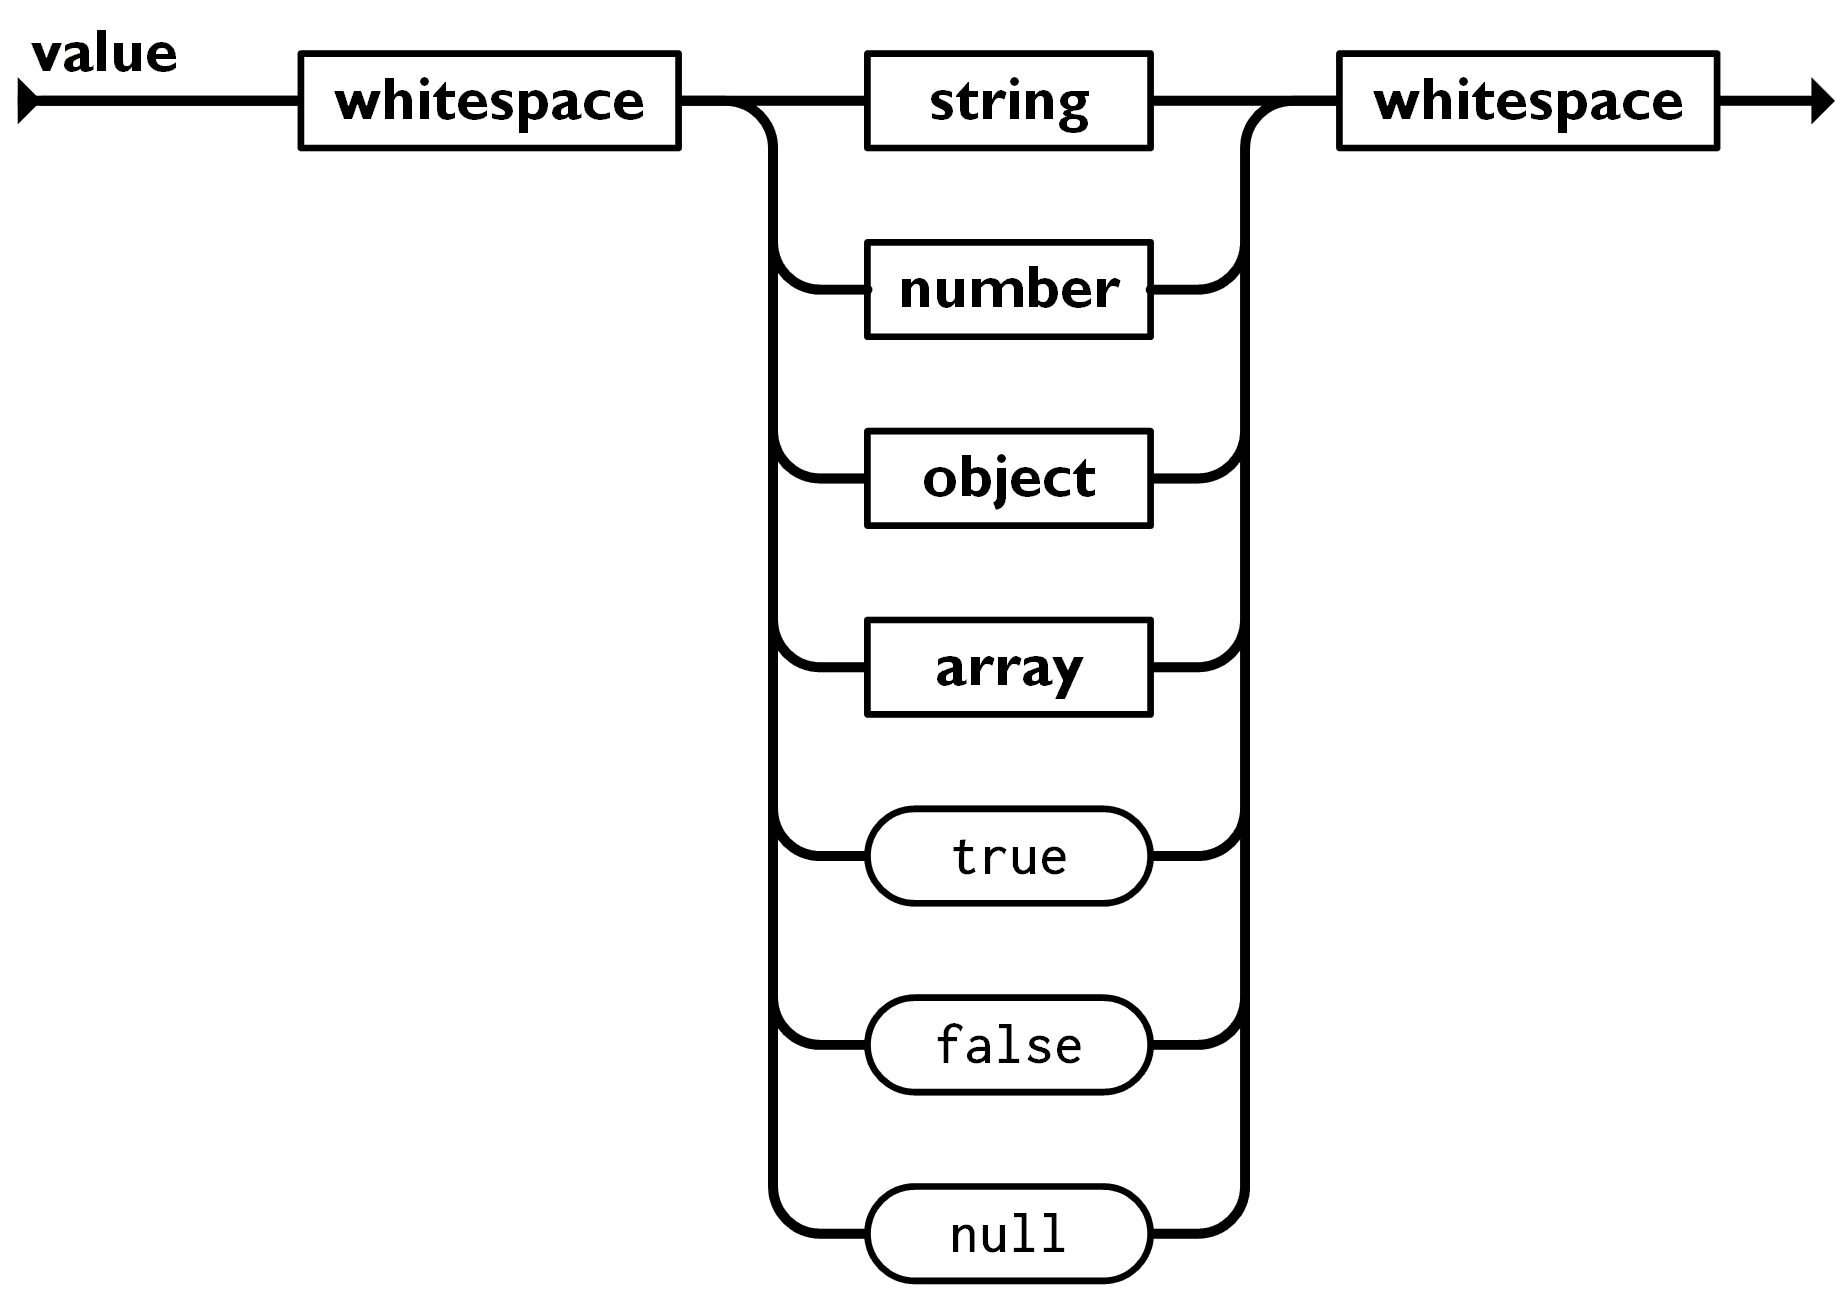
\includegraphics[width=1.0\textwidth]{Figures/json-grammar.png}
    \caption{JSON Grammar}
    \label{fig:json_grammar}
\end{figure}
\subsection{Grammar}
For the reasons previously discussed, JavaCC was chosen to create the parser. JavaCC accepts a grammar in EBNF form. It has its own file type, with the extension .jj. This file is then used to generate Java source files containing the compiler. First, tokens for quotes, commas, colons, brackets and digits were created. An integer was defined as an optional minus sign, followed by at least one digit:
\begin{verbatim}
< INTEGER : ("-")? (< DIGIT >)+ >
\end{verbatim}
A decimal is defined as an optional minus, followed by any number of digits, followed by a decimal place, followed by at least one digit:
\begin{verbatim}
< DECIMAL : ("-")? (< DIGIT >)* “.” (< DIGIT >)+ >}
\end{verbatim}
A string was defined as a quote, followed by any number of characters that are not quotes, followed by a quote:
\begin{verbatim}
< STRING : < QUOTE > (~[ "\"" ])* < QUOTE > >
\end{verbatim}
The parser was set to skip white spaces, new lines characters, and tabs. The first step was to parse JSON values, which can be a boolean, number, or string. Null values were omitted as non-technical users would not be aware of the concept of null. Boolean values were easily parsed using the true and false tokens. Integers and decimals were parsed using the BigInteger and \texttt{BigDecimal} objects respectively. These objects are built into Java, and allow very large numbers, that are above 64 bits, to be stored \cite{big_integer_big_decimal}.\par
It was worth considering whether it was logical to create new data objects specifically for the parser (some parsers have a JsonElement, JsonArray, etc objects). This can make the parser cleaner and more easier for a developer to use as an API. However since this parser is used only internally in the solution to initialise Java objects, it is not required. It would also add unnecessary overhead to the project, as the Java standard library supports all data structures required. Strings were parsed using the string token, with the opening and closing quotes removed.
\subsection{List Parsing}
The next logical thing to parse was a JSON list or array. JSON lists start with an opening square bracket \texttt{[}, have a sequence of JSON elements (can be a JSON value, another JSON list, or JSON object), and end with a closing square bracket \texttt{]}. Empty lists are allowed. The ArrayList data structure in Java was used to store the list. It is the most commonly used list data structure in Java, and allows the underlying array to be dynamically resized as elements are added \cite{array_list}. This is shown in figure \ref{fig:array_parsing}.
\begin{figure}
\centering
\caption{Array Parsing}
\label{fig:array_parsing}
\begin{verbatim}
List<Object> array() :
{
  List<Object> array = new ArrayList<Object>();
  Object element;
}
{
  < BRACKET_OPEN >
  (
    element = element()
    {
      array.add(element);
    }
    (
      < COMMA > 
      element = element()
      {
        array.add(element);
      }
    )*
  )?
  < BRACKET_CLOSE >
  {
    return array;
  }
}
\end{verbatim}
\end{figure}

\subsection{Object Parsing}
JSON objects are similar to JSON lists, however each element has both a key and corresponding value. As previously discussed, the parser would need to allow duplicate keys in objects. Usually JSON parser implementations use a map or dictionary data structure to store objects, however this can obviously not be used here. Java of course has a HashMap implementation, however two identical keys will generate the same hash, so the second key-value entry would overwrite the first. One solution would be to use both the key of the entry, and its position in the parent JSON object (such as the line number) to generate the hash. Generating hashes in this way allows the map to store multiple entries with keys of the same name, as the hash is generated off both the key and its position in the file.\par
The Google Guava library implements a HashBasedTable \cite{hash_based_table}, which allows a composite key to be generated based off of two keys. However, this data structure does not preserve insertion order, meaning object representations would lose their ordering with respect to each other. Therefore HashBasedTable can not be used in the solution. Also, this would mean any time a lookup was performed on a JSON object to get the corresponding value of a given key, both the key and its position in the file would be needed, which is inconvenient.\par
A more logical data structure for storing a JSON object is a list of key-value entries. The downside of this is that the lookup for a value of a given key is slower, O(n) in the worst case, instead of O(1) if a hash map was used. However this inefficiency is fairly insignificant, as the data structure will only be used internally. Firstly, it is used to sequentially iterate through the sequence of object representations in the file. And secondly, if the value of an entry is a JSON object, that JSON object will be used to find and initialise the correct constructor of the Java class.\par
When this is the case, the number of entries in the object will be the number of parameters in the Java class constructor, which will likely not be a large number. In other words, for what the parser is used for, there is no case where it will be required to get the value of a given key within a large JSON object, meaning there is not an issue in using this data structure.\par
The list of entries data structure for an object can be thought of as entries with pointers to the succeeding entry. A linked list stores elements by having each element have a pointer pointing to the next element. This makes it a logical choice to use as a data structure for a JSON object. It also allows the ability to distinguish between whether a list is in fact a JSON list, or JSON object, by checking if it is an instance of ArrayList or LinkedList respectively. JSON objects were parsed similarly to JSON lists, but obviously using key-value entries rather than single elements. This is shown in figure  \ref{fig:object_parsing}.
\begin{figure}
\centering
\caption{Object Parsing}
\label{fig:object_parsing}
\begin{verbatim}
List<Entry<String, Object>> object() :
{
  List<Entry<String, Object>> object =
  new LinkedList<Entry<String, Object>>();
  String key;
  Object value;
}
{
  < BRACE_OPEN >
  (
    key = string() < COLON > value = element()
    {
      object.add(Entry.of(key, value));
    }
    (
      < COMMA > 
      key = string() < COLON > value = element()
      {
        object.add(Entry.of(key, value));
      }
    )*
  )?
  < BRACE_CLOSE >
  {
    return object;
  }
}
\end{verbatim}
\end{figure}

\subsection{Parser Compilation}
At this stage the parser was almost complete. The root of any JSON parse tree is a JSON list or JSON object. The parser was set to start with initially parsing either a JSON list or JSON object, and then recursively parse the remaining structure of the JSON. The Java files for the parser were compiled from the JavaCC file and added to the project.

\section{Object Initialisation}

At this stage, the contents of a JSON file containing the representation of a program can be parsed and stored in data structures in Java. The next stage was to take this data and use it to actually initialise classes, creating object instances. The first step is to determine what classes this can be done for. As previously discussed, these types of classes are referred to as ‘blocks’, to help the understanding of non-technical users. The solution includes a standard library of blocks that can be used universally, such as the \texttt{SetAttribute} block, which sets some attribute of the program, such as its name or author. Another example is the \texttt{Wait} block, which makes the program wait a specified amount of time before the client is progressed to the next block. While these blocks serve their purpose, the project must have an API to hook into existing software libraries to maximise its usefulness. Hence, the API must allow the ability to add more blocks.\par
\subsection{Adding Custom Block Classes}
To allow custom block classes to be added, the project is compiled to a jar. Then, other projects are able to use the jar as a dependency, meaning they can add their own block classes. In a Java project, it is not possible to gain a list of all classes in the project \cite{java_classes_in_package}, even with reflection. If this was the case, it would be possible to simply make every object able to be initialised. The problem with this, even if it was possible, would be that there are many circumstances where you would not want all classes to be able to be initialised. For example, if the project has two classes of the same name but in different packages, it would be impossible to determine which class should be initialised, since the JSON representation specifies only the class name, not the package of the class. Obviously it is possible to register individual classes to be block classes, and the solution does support this. However, this is tedious if there is a large number of classes to be registered. The ability to register all classes in a package to become block classes would solve this. Java classes are organised into packages, corresponding to the folder structure of the project.
\subsection{Retrieving Classes in a Package}
It is not possible to get all classes contained in a package in Java, even with reflection. However since packages correspond to the folder structure of the source code, or of the jar if it's compiled, a workaround is possible. After some research and experimentation, two solutions were devised, depending on whether the code is compiled in a jar, or run directly from an integrated development environment. The first step is to check if the code is running in a jar, by checking if a jar file exists:
\begin{verbatim}
new File(ClassUtils.class.getProtectionDomain().getCodeSource()
.getLocation().toURI())
\end{verbatim}
If this returns true, the internal structure of the jar can be traversed using the \\\texttt{java.util.jar.JarFile} class, and the names of all .class files in a given package can be extracted as shown in figure \ref{fig:classes_in_package_jar}.
\begin{figure}
\centering
\caption{Retrieval of classes in a package in a jar}
\label{fig:classes_in_package_jar}
\begin{verbatim}
Set<Class<?>> getClassesFromJar(File jarFile, String packageName) {
  Set<Class<?>> classes = new HashSet<Class<?>>();
  try {
    JarFile file = new JarFile(jarFile);
    for (Enumeration<JarEntry> entry = file.entries(); 
entry.hasMoreElements();) {
      JarEntry jarEntry = entry.nextElement();
      String name = jarEntry.getName().replace("/", ".");
      if (name.startsWith(packageName) && name.endsWith(".class")) {
        classes.add(Class.forName(name.substring(0, name.length() - ".class".length())));
      }
    }
    file.close();
    } catch (Exception exception) {
      exception.printStackTrace();
    }
    return classes;
}
\end{verbatim}
\end{figure}
The second solution is required if the code is not compiled in a jar. This solution uses the reflections library, which extends the capabilities of standard Java reflection. It allows for runtime metadata analysis, scanning of the classpath, indexing metadata, and allows the ability to query on runtime \cite{reflections}.
At this point, the project needed to depend on this library. Apache Maven is a software project management and comprehension tool. Based on the concept of a project object model (POM), Maven can manage a project's build, reporting and documentation from a central piece of information \cite{maven}. The project was converted from a standard Java project to a Maven Java project. By adding the following XML to the project’s pom.xml file, the reflections library was automatically compiled into the project jar whenever it was built:
\begin{verbatim}
<dependency>
  <groupId>org.reflections</groupId>
  <artifactId>reflections</artifactId>
  <version>0.9.12</version>
  <scope>compile</scope>
</dependency>
\end{verbatim}
The classes in a package can be retrieved using the reflections library and \texttt{ClassLoader} as shown in figure  \ref{fig:classes_in_package_outside_jar}.
\begin{figure}
\centering
\caption{Retrieval of classes in a package outside a jar}
\label{fig:classes_in_package_outside_jar}
\begin{verbatim}
Set<Class<?>> getClassesFromClassLoader(String packageName) {
    List<ClassLoader> classLoadersList = new LinkedList<ClassLoader>();
    classLoadersList.add(ClasspathHelper.contextClassLoader());
    classLoadersList.add(ClasspathHelper.staticClassLoader());

    ConfigurationBuilder config = new ConfigurationBuilder();
    // don't exclude Object.class
    config.setScanners(new SubTypesScanner(false), new ResourcesScanner());
    // filter package
    config.filterInputsBy(new FilterBuilder()
    .include(FilterBuilder.prefix(packageName)));
    config.setUrls(ClasspathHelper.forJavaClassPath());

    return new Reflections(config).getSubTypesOf(Object.class);
}
\end{verbatim}
\end{figure}
Initially, the line
\begin{verbatim}
config.setUrls(ClasspathHelper.forJavaClassPath())
\end{verbatim}
was
\begin{verbatim}
config.setUrls(ClasspathHelper.forClassLoader(classLoadersList
.toArray(new ClassLoader[0])));
\end{verbatim}
However, the latter did not work when testing on a macOS due to differences in the Java Virtual Machine and class loader. After brief research, the corrected version was found.\par
The two solutions outlined above were combined, so that the classes in a package could be retrieved in any circumstance. This allowed the API to have a method to register all classes in a given package as block classes.
\subsection{Program Loading}
Now that the block classes could be determined, the next stage was to initialise these classes using the JSON representation. Initially, the API required setting a folder containing all JSON files to be loaded, and then a \texttt{load()} method called. However, it made more intuitive sense to have a single \texttt{load} method which takes a folder as an argument. All files contained in the folder are retrieved recursively using the method shown in figure \ref{fig:files_in_folder}.
\begin{figure}
\centering
\caption{Obtaining files in a folder recursively}
\label{fig:files_in_folder}
\begin{verbatim}
Set<File> getFiles(File folder) {
  Set<File> files = new HashSet<>();

  if (!folder.isDirectory()) {
    return files;
  }

  for (File file : folder.listFiles()) {
    if (file.isDirectory()) {
      files.addAll(getFiles(file));
    } else {
      files.add(file);
    }
  }

  return files;
}
\end{verbatim}
\end{figure}
\par
The files with a \texttt{.json} or \texttt{.blox} extension are loaded in alphabetical order, which allows non-technical users to ensure a given program gets loaded after any programs it depends on. If the file does not have valid JSON (the parsing fails) or it is not a JSON object, an \texttt{IllegalStateException} is thrown. Each key-value entry is parsed and converted into an object instance. The key is used to determine the block class used for initialisation. In order to allow maximum flexibility, the key is converted to lowercase (as block classes are registered using a lowercase key), and spaces are removed. In other words, both:
\begin{verbatim}
{
“MyObject1”:argument
}
\end{verbatim}
and...
\begin{verbatim}
{ 
“my object 1”:argument
}
\end{verbatim}
work and initialise the same object. This allows for representations to be closer to natural language. For example:
\begin{verbatim}
{
“Show home screen”:[]
}
\end{verbatim}
Will result in the initialisation of a block class named \texttt{ShowHomeScreen}.\par
Each key-value entry is then used to initialise a new object using the representations previously discussed. If a class of the given name is not found, an exception is thrown. First, a list of parameters is created. If the value of the entry is a single JSON primitive value (boolean, number or string) and not a collection (JSON list or JSON object), then that single value is extracted and added to the parameter list.\par
Values are extracted by checking if its class type is a boolean, number or string. Primitive wrapper classes  are converted into the equivalent primitive class when the type of a constructor parameter is primitive. For example, if a constructor has a parameter of type \texttt{int}, and the extracted value is of type \texttt{Integer}, the value will be converted from being an \texttt{Integer} type to an \texttt{int} type. Additionally, if a constructor parameter type is a decimal type, such as float or double, and the supplied parameter is an integer, the parameter is converted to a decimal type. This is shown in figure  \ref{fig:number_cast}.
\begin{figure}
\centering
\caption{Number Casting}
\label{fig:number_cast}
\begin{verbatim}
Object castNumber(Class<?> requiredParameter, Object parameter) {
    Class<?> suppliedParameter = parameter.getClass();

    // casts numbers to the specified type
    if (requiredParameter == double.class) {
        if (suppliedParameter == int.class || 
suppliedParameter == Integer.class) {
            return (double) ((int) parameter);
        }
    } else if (requiredParameter == float.class) {
        if (suppliedParameter == int.class || 
suppliedParameter == Integer.class) {
            return (float) ((int) parameter);
        } else if (suppliedParameter == double.class || 
suppliedParameter == Double.class) {
            return (float) ((double) parameter);
        }
    }

    return parameter;
}
\end{verbatim}
\end{figure}

These kinds of operations are performed by the Java compiler itself, which gives the language more flexibility. However, since it is obviously not possible to access elements of the Java compiler from Java runtime, these operations must be replicated at a higher level.\par

Once the parameters have been collected, a search is performed to find a constructor of the class whose parameter types match the closest to the supplied parameter types. This is done using the  algorithm shown in figure \ref{fig:best_constructor}.
\begin{figure}
\centering
\caption{Best constructor retrieval}
\label{fig:best_constructor}
\begin{verbatim}
Constructor<?> getConstructor(Class<?> clazz, List<Object> parameters, 
boolean lenient) {
    search: for (Constructor<?> c : clazz.getConstructors()) {
        int numParameters = c.getParameterTypes().length;

        // don't require array parameter
        if (numParameters > 0 && 
c.getParameterTypes()[c.getParameterTypes().length - 1].isArray()) {
            numParameters--;
        }

        // continue if not enough parameters
        if (parameters.size() < numParameters) {
            continue;
        }

        // check parameter types equal
        for (int i = 0; i < Math.min(c.getParameterTypes().length, 
parameters.size()); i++) {
            Class<?> requiredParameter = c.getParameterTypes()[i];

            // fix parameter if it is an array
            boolean array = requiredParameter.isArray() && 
            i == c.getParameterTypes().length - 1;
            requiredParameter = array ? requiredParameter.getComponentType() :
            requiredParameter;

            // if array, check all remaining parameters equal the array type
            for (int j = i; j < (array ? parameters.size() : i + 1); j++) {
                Class<?> suppliedParameter =
                castClass(parameters.get(j).getClass());

                if (!suppliedParameter.equals(requiredParameter)) {

                    // if lenient, try number casting to make parameter types match
                    if (lenient) {
                        Object number = castNumber(requiredParameter, 
                        parameters.get(j));
                        suppliedParameter = castClass(number.getClass());

                        if (suppliedParameter.equals(requiredParameter)) {
                            // update parameters with casted number
                            parameters.set(j, number);
                            continue;
                        }
                    }

                    continue search;
                }
            }
        }

        return c;
    }
    return null;
}
\end{verbatim}
\end{figure}
\subsection{Representation Flexibility}
The algorithm allows for constructors which have an array type for their final parameter to be initialised. In other words, this allows constructors such as:
\begin{verbatim}
public DisplayMessage(String... messages) {
...
}
\end{verbatim}
to be initialised using any of the following representations:
\begin{verbatim}
“DisplayMessage”: []
\end{verbatim}
(with no arguments)
\\
\begin{verbatim}
“DisplayMessage”: “Message”
\end{verbatim}
(with a single argument)
\\
\begin{verbatim}
“DisplayMessage”: [ “Line 1”, “Line 2” ]
\end{verbatim}
(with multiple arguments)
\\\\
One of the core philosophies decided whilst developing the project was to allow maximum flexibility, and enforce minimal verbosity on the non-technical user. Giving non-technical users this leeway maximises the amount of time they spend on creating programs, as they are not wasting time fixing formatting problems. It also allows the representation to be slightly closer to natural language, which as previously mentioned, is one of the goals of the project.\par

The lenient parameter of the algorithm is optional, but if specified, will make a greater effort to find the correct parameter type. This is achieved by attempting to cast number types to match the types of the constructor parameters. The solution runs the algorithm once with lenient set to false, to try and find the correct constructor with maximum precision. If the algorithm is unsuccessful, it is run again with lenient set to true. If it is still unsuccessful in finding a constructor, the provided representation does not match the class, and an \texttt{IllegalArgumentException} is thrown.\par

If the constructor found has an array type as its last parameter as mentioned, the arguments  are converted accordingly, with the last n arguments converted to a single array argument. This is achieved using the algorithm shown in figure  \ref{fig:arguments_to_array}.
\begin{figure}
\centering
\caption{Multiple argument to single array conversion}
\label{fig:arguments_to_array}
\begin{verbatim}
// if last argument of constructor is an array, convert
Class<?>[] paramTypes = constructor.getParameterTypes();
if (paramTypes.length > 0 && paramTypes[paramTypes.length - 1].isArray()) {
    List<Object> typeArray = new ArrayList<>();

    // remove parameters that form an array
    if (parameters.size() >= paramTypes.length) {
        for (int i = paramTypes.length - 1; i < parameters.size(); i++) {
            typeArray.add(parameters.get(i));
        }
        for (int i = parameters.size() - 1; i >= paramTypes.length - 1; i--) {
            parameters.remove(i);
        }
    }

    // create array and add to the parameters
    Class<?> arrayTest = paramTypes[paramTypes.length - 1];

    if (arrayTest.getComponentType().isPrimitive()) {
        parameters.add(createPrimitiveArray(typeArray, arrayTest));
    } else {
        parameters.add(typeArray.toArray((Object[]) 
Array.newInstance(arrayTest.getComponentType(), typeArray.size())));
    }
}
\end{verbatim}
\end{figure}

This is represented visually in figure  \ref{fig:arguments_to_array_visual}.

\begin{figure}
\centering
\caption{Multiple argument to single array conversion}
\label{fig:arguments_to_array_visual}
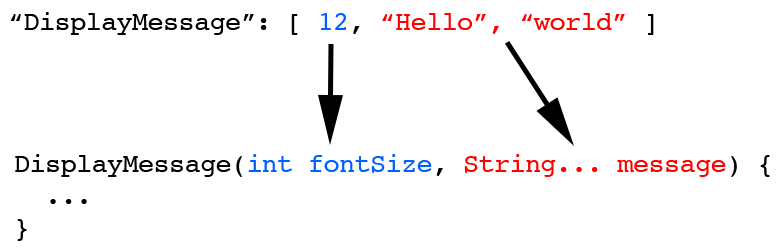
\includegraphics[width=0.7\textwidth]{Figures/array.png}
\end{figure}

Finally, the constructor is initialised and added to a list of the projects that have been initialised from the file.\par

As previously discussed, a JSON object is stored using a Java \texttt{LinkedList}, a list of key-value entries linking to each other. This means the representation can be checked to see if it is a JSON object by simply checking if it is an instance of \texttt{LinkedList}. In this case, the correct constructor for the class can be determined more accurately. This is because it is possible to search for a constructor based on the names of its parameters as well as the types of its parameters. The parameter names are checked first, as they are string types, and strings can be compared with less ambiguity and complexity than types. This is done using the algorithm displayed in figure  \ref{fig:json_object_to_java_object}.
\begin{figure}
\centering
\caption{Instantiation from JSON object representation}
\label{fig:json_object_to_java_object}
\begin{verbatim}
Map<String, Object> object = new HashMap<>();
for (Entry<String, Object> keyValue : (List<Entry<String, Object>>) value) {
    // add parameter name-value pairs to map
    object.putIfAbsent(keyValue.getKey().toLowerCase(), 
extractParameter(keyValue.getValue(), true));
}

// search for suitable constructor
constructors: for (Map.Entry<Constructor<?>, List<String>> entry : 
blockConstructors.get(blockClass).entrySet()) {
    // check if parameter names equal
    if (!object.keySet().equals(entry.getValue().stream().collect(Collectors.toSet()))) {
        continue;
    }

    // clear parameters from previous attempts
    parameters.clear();

    // check if parameter types equal
    Class<?>[] paramTypes = entry.getKey().getParameterTypes();
    List<String> paramNames = entry.getValue();

    for (int i = 0; i < paramTypes.length; i++) {
        String paramName = paramNames.get(i);
        Object suppliedParam = object.get(paramName);
        Class<?> suppliedClass = castClass(suppliedParam.getClass());

        // nested block
        if (suppliedParam instanceof LinkedList) {
            suppliedParam = getBlock(paramTypes[i], suppliedParam);
        } else {
            // cast number to match type
            suppliedParam = castNumber(paramTypes[i], suppliedParam);
        }

        // check parameter types equal
        if (!suppliedClass.equals(paramTypes[i])) {
            continue constructors;
        }

        // add parameter
        parameters.add(suppliedParam);
    }

    // both parameter names and type equal, save the discovered constructor and stop searching
    constructor = entry.getKey();
    break;
}
\end{verbatim}
\end{figure}
First, the list of entries is converted to a map (since this JSON object will never need to have keys with the same entries). The keys are converted to lowercase so that they can be compared to the parameters names of the constructor with case insensitivity.\par

The JSON object keys must now be compared to the parameter names of the block classes’ constructors. It is not possible to determine constructor parameter names in Java within the standard Java library, even using reflection \cite{java_constructor_parameter_names}. Again, an external library must be used. ASM is an all purpose Java bytecode manipulation and analysis framework. It can be used to modify existing classes or to dynamically generate classes, directly in binary form \cite{asm}. It enables the ability to extract constructor parameter names using the algorithm shown in figure  \ref{fig:constructor_parameter_names}.
\begin{figure}
\centering
\caption{Retrieval of constructor parameter names}
\label{fig:constructor_parameter_names}
\begin{verbatim}
List<String> getConstructorParameterNames(Constructor<?> constructor) {
    Class<?> declaringClass = constructor.getDeclaringClass();
    ClassLoader declaringClassLoader = declaringClass.getClassLoader();

    Type declaringType = Type.getType(declaringClass);
    String constructorDescriptor = Type.getConstructorDescriptor(constructor);
    String url = declaringType.getInternalName() + ".class";

    InputStream classFileInputStream = declaringClassLoader.getResourceAsStream(url);
    if (classFileInputStream == null) {
        throw new IllegalArgumentException("The constructor's class loader cannot find the bytecode that defined the constructor's class (URL: " + url + ")");
    }

    ClassNode classNode = null;
    try {
        try {
            classNode = new ClassNode();
            ClassReader classReader = new ClassReader(classFileInputStream);
            classReader.accept(classNode, 0);
        } finally {
            classFileInputStream.close();
        }
    } catch (Exception exception) {
        throw new IllegalArgumentException("Error getting constructor parameter names for " + constructor.getClass());
    }

    List<MethodNode> methods = classNode.methods;
    for (MethodNode method : methods) {
        if (method.name.equals("<init>") && method.desc.equals(constructorDescriptor)) {
            Type[] argumentTypes = Type.getArgumentTypes(method.desc);
            List<String> parameterNames = new ArrayList<String>(argumentTypes.length);

            List<LocalVariableNode> localVariables = method.localVariables;
            for (int i = 0; i < argumentTypes.length; i++) {
                // the first local variable actually represents the "this" object
                parameterNames.add(localVariables.get(i + 1).name);
            }

            return parameterNames;
        }
    }

    return null;
}
\end{verbatim}
\end{figure}
The ASM library was added to the project build in a similar fashion to the reflections library, by adding the following XML to the projects pom.xml:
\begin{verbatim}
<dependency>
    <groupId>org.ow2.asm</groupId>
    <artifactId>asm</artifactId>
    <version>7.1</version>
</dependency>
<dependency>
    <groupId>org.ow2.asm</groupId>
    <artifactId>asm-tree</artifactId>
    <version>7.1</version>
</dependency>
\end{verbatim}
The parameters names for a given class’ constructors are cached for efficiency when the class is registered as a block class. The cache is accessed when trying to find a constructor of a given block class with given parameter names. Once a constructor that has parameter names that match the keys of the JSON object is found, the types of the parameters are compared to the values of the JSON object. If the types match, the constructor is used to initialise a new instance of the class.\par

As previously discussed, JSON object representations of Java objects support nested objects. For example, the following case initialises a new instance of the MyObject1, using a constructor with a parameter of type MyObject2:
\begin{verbatim}
“MyObject1”:{
  “MyObject2”:{
  ...
  }
}
\end{verbatim}
This is implemented by recursively calling the method to initialise a block if a value inside a JSON object is another JSON object.

\section{API}

In order to maximise the usefulness of initialised classes, an API was included to increase the capabilities a developer has to design classes specifically to be used by non-technical users. Once a file is parsed and deserialised to objects, these objects are stored in a list, which is stored within a \texttt{Script} object. This object is used to run the program the file represents. The reason for naming the class \texttt{Script} rather than \texttt{Program} is to reflect the fact that the program will usually be small but flexible, and be dynamically interchangeable in runtime, much like scripts are. However since these programs are compiled, not interpreted, from a technical perspective they are still programs. The API also allows for programs to be loaded and unloaded during runtime.\par

\subsection{Block Class Interfaces}
The \texttt{Block} interface can optionally be implemented by classes registered as block classes. This allows the class to override the methods \texttt{onLoad} and \texttt{onUnload}, which are called when the program is loaded and unloaded respectively. It also gives the class access to its parent \texttt{Script} objects, which can be used to access other blocks in the program. This allows multiple blocks to be used together to provide combined functionality.\par

When programs are run, they often provide some functionality to the client. When this is the case, the idea is that the client progresses through the program one block at a time, with each block providing some behaviour for the client. Client is referred to here in abstract terms. The definition depends on what the project is being applied to. In the case of some graphical interface, the client will represent the user using the interface. In the case of a game, the client will be a player of the game. When the API is initialised, the desired class to represent the client is supplied as a generic type.\par

The \texttt{ClientBlock} interface is an extension of the \texttt{Block} interface which allows classes to implement these behaviours. The \texttt{onEnter} and \texttt{onExit} can be overridden to detect when the client enters and exits the block respectively. After the client has entered the block, it can be progressed to the next block using the \texttt{progress} method. The \texttt{onEnterScript} and \texttt{onExitScript} can be overridden to detect when a client enters and exits the program respectively. In other words, when they enter and exit any block in the program.\par

Any class can be used as a block class; they do not need to implement any interfaces from the API. However, classes that do not implement any of these interfaces will have limited functionality, and will most likely be used as data classes. Classes that implement \texttt{Block} are able to access their parent program, and classes that implement \texttt{ClientBlock} are able to provide behaviour to the client when they run the program. Hence there are three main types of block classes: data blocks that have no behaviour, program blocks that have behaviour that affects the program and other blocks within the program, and client blocks that have behaviour that affects the client.

%\chapter{Testing}

\section{API Tests}

\section{Representation Tests}

 
%\chapter{Use Cases}

\section{Artificial Intelligence}

\section{Game Modding} 

%----------------------------------------------------------------------------------------
%	THESIS CONTENT - APPENDICES
%----------------------------------------------------------------------------------------

\appendix % Cue to tell LaTeX that the following "chapters" are Appendices

% Include the appendices of the thesis as separate files from the Appendices folder
% Uncomment the lines as you write the Appendices

% Appendix A

\chapter{Frequently Asked Questions} % Main appendix title

\label{AppendixA} % For referencing this appendix elsewhere, use \ref{AppendixA}

\section{How do I change the colors of links?}

The color of links can be changed to your liking using:

{\small\verb!\hypersetup{urlcolor=red}!}, or

{\small\verb!\hypersetup{citecolor=green}!}, or

{\small\verb!\hypersetup{allcolor=blue}!}.

\noindent If you want to completely hide the links, you can use:

{\small\verb!\hypersetup{allcolors=.}!}, or even better: 

{\small\verb!\hypersetup{hidelinks}!}.

\noindent If you want to have obvious links in the PDF but not the printed text, use:

{\small\verb!\hypersetup{colorlinks=false}!}.

%\include{Appendices/AppendixB}
%\include{Appendices/AppendixC}

%----------------------------------------------------------------------------------------
%	BIBLIOGRAPHY
%----------------------------------------------------------------------------------------

\printbibliography[heading=bibintoc]

%----------------------------------------------------------------------------------------

\end{document}  
